\begin{frame}{Experimentos}
    \begin{itemize}
        \item Implementação: rmM-tree binária e rmM-tree k-ária;
        \item Validação das respostas;
        \item Testes de desempenho.
    \end{itemize}
\end{frame}



\begin{frame}{Experimentos: validação}
    
    \begin{figure}[h!]
        \centering
        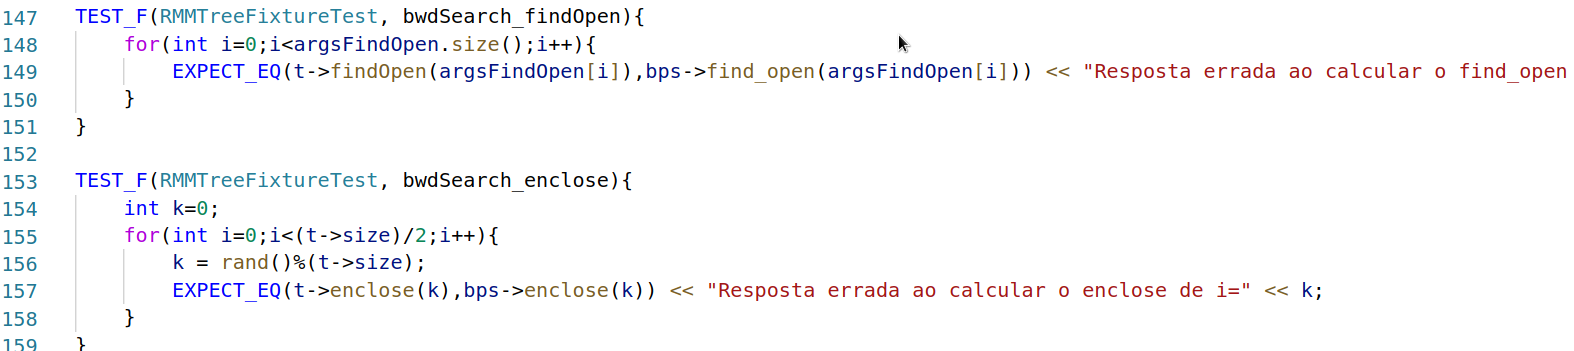
\includegraphics[scale=0.25]{images/unit_tests.png}\\
        \caption{Testes unitários para as operações \textit{findopen} e \textit{enclose}}
    \end{figure} 
\end{frame}

\begin{frame}{Experimentos: desempenho}
    
    \begin{figure}[h!]
        \centering
        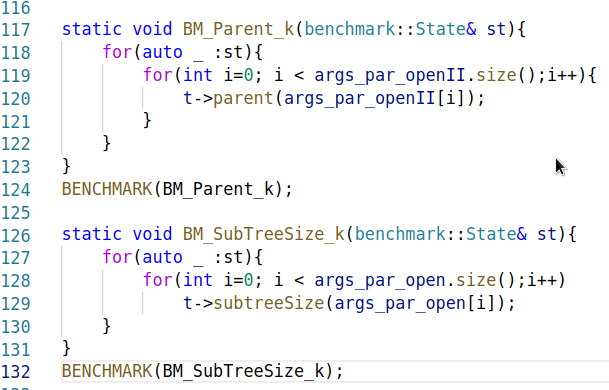
\includegraphics[scale=0.35]{images/benchmar.png}\\
        \caption{Testes de desempenho para as operações \textit{parent} e \textit{subtreeSize}}
    \end{figure} 
\end{frame}


